% Document settings
\documentclass[a4paper,11pt]{article}

% Packages
  % math formulas
\usepackage{amsmath,amsthm,amssymb}
  % graphics
\usepackage{graphicx}
\usepackage{wrapfig}
  % plots
\usepackage{pgfplots}
  % other
\usepackage[warn]{mathtext}
\usepackage{cmap}
\usepackage[T1,T2A]{fontenc}
\usepackage[utf8]{inputenc}
\usepackage[english,russian]{babel}

% Package settings
%% graphicx
\graphicspath{{Pictures/}}
\DeclareGraphicsExtensions{.pdf,.png,.jpg}
%% pgfplots
\pgfplotsset{width=10cm,compat=1.9}
% Title
\title{Отчет о выполнении работы №2.1.6\\Эффект Джоуля-Томпсона}
\author{Воейко Андрей Александрович, Б01-109}
\date{Долгопрудный, 2022}

% Document
\begin{document}
\maketitle
\newpage
%%%%% АННОТАЦИЯ %%%%%
\section{Аннотация.}
В работе определяется изменение температуры углекислого газа при протекании через малопроницаемую перегородку при разных начальных значениях давления и температуры. Также вычисляются коэффиценты $a$ и $b$ уравнения Ван-Дер-Ваальса.
%%%%% ТЕОРЕТИЧЕСКИЕ СВЕДЕНИЯ %%%%%
\section{Теоретические сведения.}
Эффект Джоуля-Томпсона -- это изменение температуры газа, медленно перетекающего из области высокого давления в область низкого давления в условиях хорошей тепловой изоляции. Возникает он из-за того, что сближаясь, молекулы (или атомы) газа начинают взаимодействовать друг с другом, а именно отталкиваться, что приводит к увеличению потенциальной энергии их взаимодействия, и, как следствие, уменьшению их кинетической энергии, то есть температуры. В разреженных газах, по своим свойствам приближающимся к идеальным, такой эффект не наблюдается. Таким образом, эффект Джоуля-Томпсона демонстрирует отличие газа от идеального.\\
В работе исследуется изменение температуры газа при медленном течении по трубке с пористой перегородкой. Трубка 1 хорошо изолированна. Газ из области повышенного давления $P_{1}$ проходит в область с атмосферным давлением $P_{2}$. Перпад давления $\Delta P = P_{1} - P_{2}$ заметно даже при небольшой скорости течения газа в трубке ввиду большого сопротивления каналов. Величина эффекта Джоуля-Томпсона может быть определена по разности температуры до и после перегородки.\\
Рассмотрим стационарный поток газа между двумя сечениями $I$ и $II$, до и после перегородки соответственно. Для определенности рассмотрим прошедший через трубку 1 моль углекислого газа, молярная масса которого составляет $\mu$ моль. Молярные объемы газа, его давления и отнесенные к молю внутренние энергии в сечениях $I$ и $II$ обозначим соответственно $V_{1}$, $P_{1}$, $U_{1}$ и $V_{2}$, $P_{2}$, $U_{2}$. Для того, чтобы ввести газ объемом $V_{1}$ в трубку, нужно совершить работу $A_{1} = P_{1} V_{1}$. При прохождении через сечение 2, газ совершает работу. Поскольку через боковые стенки не происходит обмена теплом, справедлива формула:\\
\begin{equation}    \label{eq1}
  A_{1} - A_{2} = \left(U_{2} + \frac{\mu v_{2}^{2}}{2}\right) - \left(U_{1} + \frac{\mu v_{1}^{2}}{2}\right).
\end{equation}
Теперь найдем изменение энтальпии. Подставляя вместо $PV$ соотвествующую работу $A$, получаем:
\begin{equation}    \label{eq2}
  H_{1} - H_{2} = \left(U_{1} + P_{1}V_{1}\right) - \left(U_{2} + P_{2}V_{2}\right) = \frac{1}{2} \mu \left(v_{2}^{2} - v_{1}^{2}\right).
\end{equation}
Процесс Джоуля-Томпсона в чистом виде осуществляется только в том случае, если правой частью можно пренебречь. У нас пока нет критериев, позволяющих точно это установить, но тем не менее предположим, что это так. Тогда коэффицент Джоуля-Томпсона равен:\\
\begin{equation}    \label{eq3}
  \mu_{д-т} = \frac{\Delta T}{\Delta P} \approx \frac{(2a/RT) - b}{C_{p}}.
\end{equation}
\section{Экспериментальная установка.}
\subsection{Используемые приборы.}
В работе используются:
\begin{itemize}
  \item Трубка с пористой перегородкой.
  \item Труба Дьюара.
  \item Термометры.
  \item Дифференциальная термопара.
  \item Микровольтметр.
  \item Балластный баллон.
  \item Манометр.
\end{itemize}
\subsection{Описание установки.}
Схема установки изображена на рисунке~1. Основным элементом установки является трубка~1 с пористой перегородкой~2, через которую пропускается ииследуемый газ. Трубка имеет длину $80 \ мм$ и сделана из нержавеющей стали, обладающей, как известно, малой теплопроводностью. Диаметр трубки $d = 33\ мм$, толщина стенок $0,2\ мм$. ПОристая перегородка расположена в конце трубки и представляет собой стеклянную пористую пробку со множеством узких и длинных каналов. Пористость и толщина пробки ($l = 5\ мм$) подобраны так, чтобы обеспечить оптимальный поток газа при перепаде давлений $\Delta P \leq 4\ атм$ (расход газа составляет примерно $10\ \frac{см^{3}}{с}$); при этом в результате эффекта Джоуля-Томпсона создается достаточная разность температур.\\
Углекислый газ поступает под повышенным давлением в трубку через змеевик~5 из балластного баллона~6. Медный змеевик омывается модой и нагревает медленно протекающий через него газ до темепарутры воды в термостате. Температура воды измеряется термометром $T_{в}$ помещенном в термостате. Требуемая температура воды устанавливается и поддерживается во время эксперимента ври помощи контактного термометра
\begin{center}
  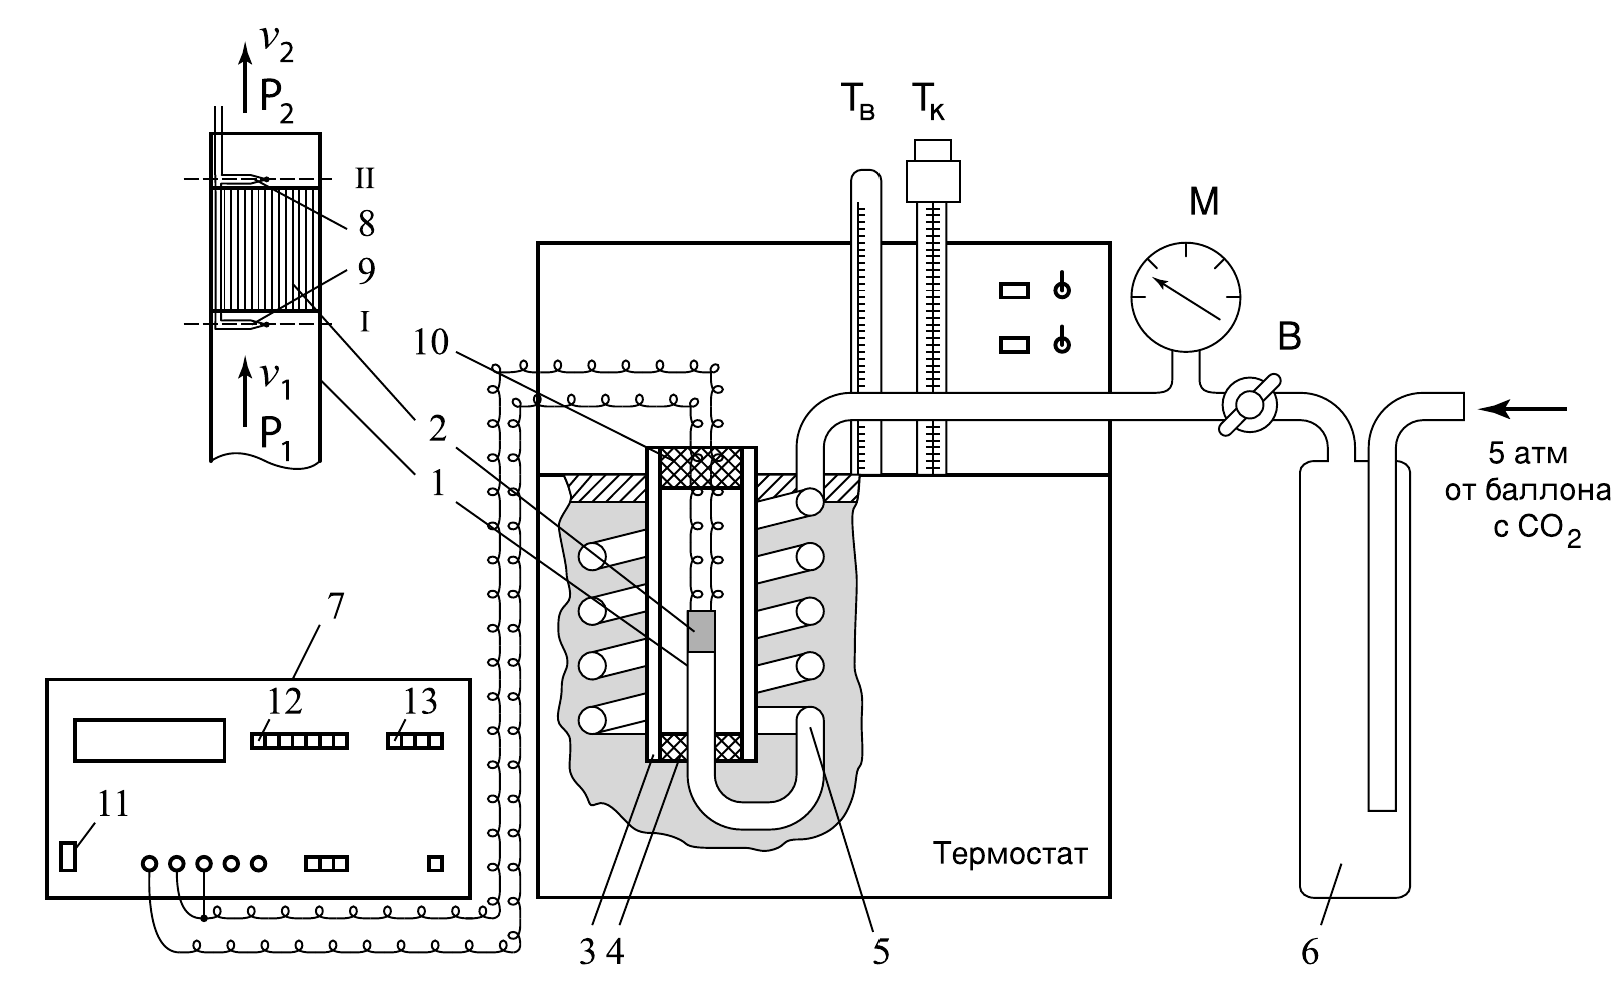
\includegraphics[scale = 0.35]{scheme1.png}\\
  Рис. 1: Схема экспериментальной установки.
\end{center}
$T_{к}$.\\
Давление газа в трубке измеряеся манометром $М$ и регулируется вентилем $В$ (при открытии вентиля $В$, т. е. при повороте ручки против часовой стрелки, давление $P_{1}$ повышается). Манометр $М$ измеряет разность между давлием внутри трубки и наружным (атмосферным) давлением. Так как углекислый газ после пористой перегородки выходит в область с атмосферным двалением $P_{2}$, то этот манометр непосредственно измеряет перепад давления на входе и на выходе трубки $\Delta P = P_{1} - P_{2}$.\\
Разность температур газа до перегородки и посде нее измеряется дифференицальной термопарой медь -- коснтантан. Конастантановая проволока диаметром $0,01\ мм$ соединяет спаи~8 и 9, а медные проволоки (того же диаметра) подсоединены к цифровому вольтметру~7. Отвод тепла через проволоку столь малого сечения пренебрежимо мал. Для уменьшения теплоотвода трубка с пористой перегородкой помещена в трубку Дьюара~3, стенки которой посеребрены, для уменьшения теплоотдачи, связанной с излучением. Для уменьшения топлоотдачи, связанной с излучением. Для уменьшения теплоотдачи за счет конвекции один конец трубы Дьюара уплотнен кольцом~4, а другой закрыт пробкой~10 из пенопласта. Такая пробка практичеси не создает перепада давлений между внутренней полостью трубы и атмосферой.
\section{Результаты измерений и обработка данных.}
\subsection{Измерения разности в зависимости от температуры.}
Проведем четыре серии измерений зависимости изменения температуры от подаваемого давления при четырех рахных температурах. Результаты измерений приведены в таблице~\ref{table:tab1}.
% Табл. 1 {{{
\begin{table}[h!]
\centering
\begin{tabular}{ ||c|c|c|c|c|| }
  \hline
  \multicolumn{4}{||c|}{Серия измерений} & 1 \\
  \hline
  № & $\Delta P$, $атм$ & $U_{тп}$, $мкВ$ & $\Delta T$, $^{\circ}C$ & $T$, $^{\circ}C$ \\
  \hline
  1 & $4,0$ & $-150 \pm 1$ & $3,69 \pm 0,02$ & $20,20 \pm 0,01$ \\
  2 & $3,5$ & $-128 \pm 1$ & $3,14 \pm 0,02$ & $20,23 \pm 0,01$ \\
  3 & $3,0$ & $-107 \pm 1$ & $2,64 \pm 0,02$ & $20,24 \pm 0,01$ \\
  4 & $2,5$ &  $-87 \pm 1$ & $2,14 \pm 0,02$ & $20,26 \pm 0,01$ \\
  5 & $2,0$ &  $-60 \pm 1$ & $1,47 \pm 0,02$ & $20,33 \pm 0,01$ \\
  \hline
  \hline
  \multicolumn{4}{||c|}{Серия измерений} & 2 \\
  \hline
  № & $\Delta P$, $атм$ & $U_{тп}$, $мкВ$ & $\Delta T$, $^{\circ}C$ & $T$, $^{\circ}C$ \\
  \hline
  1 & $4,0$ & $-147 \pm 1$ & $3,53 \pm 0,02$ & $30,06 \pm 0,01$ \\
  2 & $3,5$ & $-121 \pm 1$ & $2,91 \pm 0,02$ & $30,09 \pm 0,01$ \\
  3 & $3,0$ &  $-99 \pm 1$ & $2,38 \pm 0,02$ & $30,08 \pm 0,01$ \\
  4 & $2,5$ &  $-79 \pm 1$ & $1,90 \pm 0,02$ & $30,08 \pm 0,01$ \\
  5 & $2,0$ &  $-56 \pm 1$ & $1,35 \pm 0,02$ & $30,06 \pm 0,01$ \\
  \hline
  \hline
  \multicolumn{4}{||c|}{Серия измерений} & 3 \\
  \hline
  № & $\Delta P$, $атм$ & $U_{тп}$, $мкВ$ & $\Delta T$, $^{\circ}C$ & $T$, $^{\circ}C$ \\
  \hline
  1 & $4,0$ & $-141 \pm 1$ & $3,32 \pm 0,02$ & $40,07 \pm 0,01$ \\
  2 & $3,5$ & $-122 \pm 1$ & $2,87 \pm 0,02$ & $40,07 \pm 0,01$ \\
  3 & $3,0$ &  $-99 \pm 1$ & $2,33 \pm 0,02$ & $40,08 \pm 0,01$ \\
  4 & $2,5$ &  $-79 \pm 1$ & $1,86 \pm 0,02$ & $40,07 \pm 0,01$ \\
  5 & $2,0$ &  $-60 \pm 1$ & $1,41 \pm 0,02$ & $40,00 \pm 0,01$ \\
  \hline
  \hline
  \multicolumn{4}{||c|}{Серия измерений} & 4 \\
  \hline
  № & $\Delta P$, $атм$ & $U_{тп}$, $мкВ$ & $\Delta T$, $^{\circ}C$ & $T$, $^{\circ}C$ \\
  \hline
  1 & $4,0$ & $-131 \pm 1$ & $3,03 \pm 0,02$ & $50,10 \pm 0,01$ \\
  2 & $3,5$ & $-109 \pm 1$ & $2,51 \pm 0,02$ & $50,06 \pm 0,01$ \\
  3 & $3,0$ &  $-90 \pm 1$ & $2,08 \pm 0,02$ & $50,05 \pm 0,01$ \\
  4 & $2,5$ &  $-72 \pm 1$ & $1,66 \pm 0,02$ & $50,05 \pm 0,01$ \\
  5 & $2,0$ &  $-51 \pm 1$ & $1,18 \pm 0,02$ & $50,05 \pm 0,01$ \\
  \hline
\end{tabular}
    \caption{Зависимость изменения температуры от подаваемого давления в первой серии экспериментов.}
\label{table:tab1}
\end{table}\newline
% }}}
Во всех случаях разброс температур менее одного процента, что позволяет считать её постоянной для кождой серии измерений.
\subsection{Графики зависимости $\Delta T$ от $\Delta P$.}
Построим график зависимости изменения температуры от разности давлений для всех четырех серий измерений. Проведем прямые через все четыре графика.
% Граф. 1 {{{
\begin{center}
\begin{tikzpicture}
\begin{axis}[
    xlabel = {$\Delta P$},
    ylabel = {$\Delta T$},
    xmin = 1.5,
    xmax = 4.5,
    ymin = 0.91,
    ymax = 4.26,
    grid = major,
    minor tick num = 6
]
\addplot[
    mark size=2pt,
    only marks,
    blue,
]
table {
    x   y
    4   3.69
    3.5 3.14
    3   2.64
    2.5 2.14
    2   1.47
};
\addplot[
    no marks,
    % yes, Marx
    black,
]
table {
    x   y
    4.5 4.26
    1.5 0.91
};
% \addplot[blue, samples = 300] { sqrt(4 - x^2) };
\end{axis}
\end{tikzpicture}\\
Рисунок 2: Зависимость изменения температур от разницы давлений в первой серии измерений.\\
\end{center}
% }}}
% Граф. 2 {{{
\begin{center}
\begin{tikzpicture}
\begin{axis}[
    xlabel = {$\Delta P$},
    ylabel = {$\Delta T$},
    xmin = 1.5,
    xmax = 4.5,
    ymin = 0.787,
    ymax = 4.05,
    grid = major,
    minor tick num = 6
]
\addplot[
    mark size=2pt,
    only marks,
    red,
]
table {
    x   y
    4   3.53
    3.5 2.91
    3   2.38
    2.5 1.90
    2   1.35
};
\addplot[
    no marks,
    % yes, Marx
    black,
]
table {
    x   y
    4.5 4.03
    1.5 0.798
};
% \addplot[blue, samples = 300] { sqrt(4 - x^2) };
\end{axis}
\end{tikzpicture}\\
Рисунок 3: Зависимость изменения температур от разницы давлений во второй серии измерений.\\
\end{center}
% }}}
% Граф. 3 {{{
\begin{center}
\begin{tikzpicture}
\begin{axis}[
    xlabel = {$\Delta P$},
    ylabel = {$\Delta T$},
    xmin = 1.5,
    xmax = 4.5,
    ymin = 0.91,
    ymax = 3.80,
    grid = major,
    minor tick num = 6
]
\addplot[
    mark size=2pt,
    only marks,
    magenta,
]
table {
    x   y
    4   3.32
    3.5 2.87
    3   2.33
    2.5 1.86
    2   1.41
};
\addplot[
    no marks,
    % yes, Marx
    black,
]
table {
    x   y
    4.5 3.80
    1.5 0.91
};
% \addplot[blue, samples = 300] { sqrt(4 - x^2) };
\end{axis}
\end{tikzpicture}\\
Рисунок 4: Зависимость изменения температур от разницы давлений в третьей серии измерений.\\
\end{center}
% }}}
% Граф. 4 {{{
\begin{center}
\begin{tikzpicture}
\begin{axis}[
    xlabel = {$\Delta P$},
    ylabel = {$\Delta T$},
    xmin = 1.5,
    xmax = 4.5,
    ymin = 0.73,
    ymax = 3.46,
    grid = major,
    minor tick num = 6
]
\addplot[
    mark size=2pt,
    only marks,
    green,
]
table {
    x   y
    4   3.03
    3.5 2.51
    3   2.08
    2.5 1.66
    2   1.18
};
\addplot[
    no marks,
    % yes, Marx
    black,
]
table {
    x   y
    4.5 3.46
    1.5 0.73
};
\end{axis}
\end{tikzpicture}\\
Рисунок 5: Зависимость изменения температур от разницы давлений в четвертой серии измерений.\\
\end{center}
% }}}
Вычислим коэффицент угла наклона графиков для каждой серии измерений методом наименьших квадратов.
$$k_{1} = 1,12 \pm 0,02\ \frac{К}{атм}.$$
$$k_{2} = 1,07 \pm 0,02\ \frac{К}{атм}.$$
$$k_{3} = 0,96 \pm 0,01\ \frac{К}{атм}.$$
$$k_{4} = 0,91 \pm 0,01\ \frac{К}{атм}.$$
Таким образом,
$$\mu_{1} = 1,12 \pm 0,02\ \frac{К}{атм} = 1,10 \cdot 10^{-5} \pm 0,02 \cdot 10^{-5}\ \frac{^{\circ}С}{Па},$$
$$\mu_{2} = 1,07 \pm 0,02\ \frac{К}{атм} = 1,06 \cdot 10^{-5} \pm 0,02 \cdot 10^{-5}\ \frac{^{\circ}С}{Па},$$
$$\mu_{3} = 0,96 \pm 0,01\ \frac{К}{атм} = 0,95 \cdot 10^{-5} \pm 0,01 \cdot 10^{-5}\ \frac{^{\circ}С}{Па},$$
$$\mu_{4} = 0,91 \pm 0,01\ \frac{К}{атм} = 0,90 \cdot 10^{-5} \pm 0,01 \cdot 10^{-5}\ \frac{^{\circ}С}{Па}.$$
\subsection{Поиск коэффицентов $a$ и $b$ Ван-дер-Ваальса.}
Согласно формуле~\ref{eq3},
$$\mu_{д-т} \approx \frac{\frac{2a}{RT} - b}{C_{p}} = \frac{2a}{R C_{p}} \frac{1}{T} - \frac{b}{C_{p}}.$$
Таким образом, построив график $\mu_{д-т}\left(\frac{1}{T}\right)$ и аппроксимировав его к прямой $\mu_{д-т} = \alpha + \beta \frac{1}{T}$, мы по этим коэффицентам $\alpha$ и $\beta$ сможем найти коэффиценты $b$ и $a$, соотвественно.
% Граф. 4 {{{
\begin{center}
\begin{tikzpicture}
\begin{axis}[
    xlabel = {$1/T, \cdot 10^{-3}\ \frac{1}{К}$},
    ylabel = {$\mu_{д-е}, \cdot 10^{-5}\ \frac{К}{Па}$},
    xmin = 3.0,
    xmax = 3.5,
    ymin = 0.833,
    ymax = 1.176,
    grid = major,
    minor tick num = 6
]
\addplot[
    mark size=2pt,
    only marks,
    black,
]
table {
    x    y
    3.41 1.10
    3.19 0.95
};
\addplot[
    mark size=2pt,
    only marks,
    magenta,
]
table {
    x    y
    3.30 1.06
    3.09 0.90
};
\addplot[
    no marks,
    % yes, Marx
    black,
]
table {
    x   y
    3.5 1.176
    3.0 0.833
};
\end{axis}
\end{tikzpicture}\\
Рисунок 5: Зависимость изменения температур от разницы давлений в четвертой серии измерений.\\
\end{center}
% }}}
После аппроксимации получаем:
$$\alpha = -\frac{b}{C_{p}} = -1,2 \cdot 10^{-5} \pm 0,2 \cdot 10^{-5} \Rightarrow b = 36 \pm 6\ \frac{см^{3}}{моль}.$$
$$\beta = \frac{2a}{RC_{p}} = 0,0069 \pm 0,0006 \Rightarrow a = 0,41 \pm 0,04\ \frac{Н \cdot м^{4}}{моль^{2}}.$$
\section{Выводы.}
В ходе работы были найдены коэффценты Джоуля-Томпсона для четырех различных температур.
$$\mu_{1} = 1,12 \pm 0,02\ \frac{К}{атм} = 1,10 \cdot 10^{-5} \pm 0,02 \cdot 10^{-5}\ \frac{^{\circ}С}{Па},$$
$$\mu_{2} = 1,07 \pm 0,02\ \frac{К}{атм} = 1,06 \cdot 10^{-5} \pm 0,02 \cdot 10^{-5}\ \frac{^{\circ}С}{Па},$$
$$\mu_{3} = 0,96 \pm 0,01\ \frac{К}{атм} = 0,95 \cdot 10^{-5} \pm 0,01 \cdot 10^{-5}\ \frac{^{\circ}С}{Па},$$
$$\mu_{4} = 0,91 \pm 0,01\ \frac{К}{атм} = 0,90 \cdot 10^{-5} \pm 0,01 \cdot 10^{-5}\ \frac{^{\circ}С}{Па}.$$
Для первой и третьей серий измерений есть табличные значения, составляющие соответственно $\mu_{1}^{(табл)} = 1,105$ и $\mu_{3}^{(табл)} = 0,958$ для давления порядка $\approx 1\ атм$, что позволяет считать наши измерения вполне точными, так как оба значения лежат в пределах погрешности.\\
А вот построение графика выявило, что оставшиеся два измерения (первое и третье слева на графике, выделены светлым цветом) проведены с ошибкой, в результате чего поиск коэффицентов $a$ и $b$ уравнения Ван-дер-Ваальса был произведен с большой погрешностью в $25\%$ для $a$ и $17\%$ для $b$.\\
Сами значения составили:
$$a = 0,41 \pm 0,04\ \frac{Н \cdot м^{4}}{моль^{2}},$$
$$b = 36 \pm 6\ \frac{см^{3}}{моль}.$$
Табличные же значения этих величин составляют соответственно $a^{(табл)} = 0,37\ \frac{Н \cdot м^{4}}{моль^{2}}$ и $b^{(табл)} = 43\ \frac{см^{3}}{моль}$, что укладывается в погрешность, но это можно скорее считать счастливым стечением обстоятельств, чем подтверждением результатов вычисления.
\end{document}
